\noindent\begin{minipage}{\linewidth}
\centering
\resizebox{\linewidth}{!}{\sffamily
{(a)} \begin{tabular}{c|c|c|c|c|c|c}
\texttt{\#78} (284 nt) & Boltzmann prob. & ensemble defect & struct. distance & energy gap & & \\
``Mat - Lot 2-2 B'' & $p(\vecystar \mid \vecx)$$(\uparrow)$ & \NED$(\vecx, \vecystar)$$(\downarrow)$ & $d(\MFE(\vecx), \vecystar)$$(\downarrow)$ & \DDG$(\vecx, \vecystar)$$(\downarrow)$ & is \MFE & is uMFE \\
\hline
EliteDesign ($N=500$) & \textbf{0.0073} & \textbf{0.042} & \textbf{4} & \textbf{2.4 kcal/mol} & No & No \\
SamplingDesign & $2.35 \times 10^{-4}$ & 0.157 & \textbf{4} & 3.3 kcal/mol & No & No \\
\hline
Probability ceiling & 0.0184 & --- & --- & --- & --- & --- \\
\end{tabular}}\\[5pt]
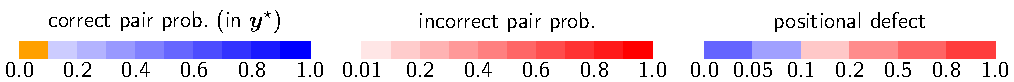
\includegraphics[width=0.9\linewidth]{figures/structures/legend}\\[3pt]
{\sffamily\small
\begin{tabular}{@{}c@{\hspace{0.02\linewidth}}c@{}}
(b) Target structure \vecystar & (c) \MFE structure of EliteDesign ($N=500$) \\[1pt]
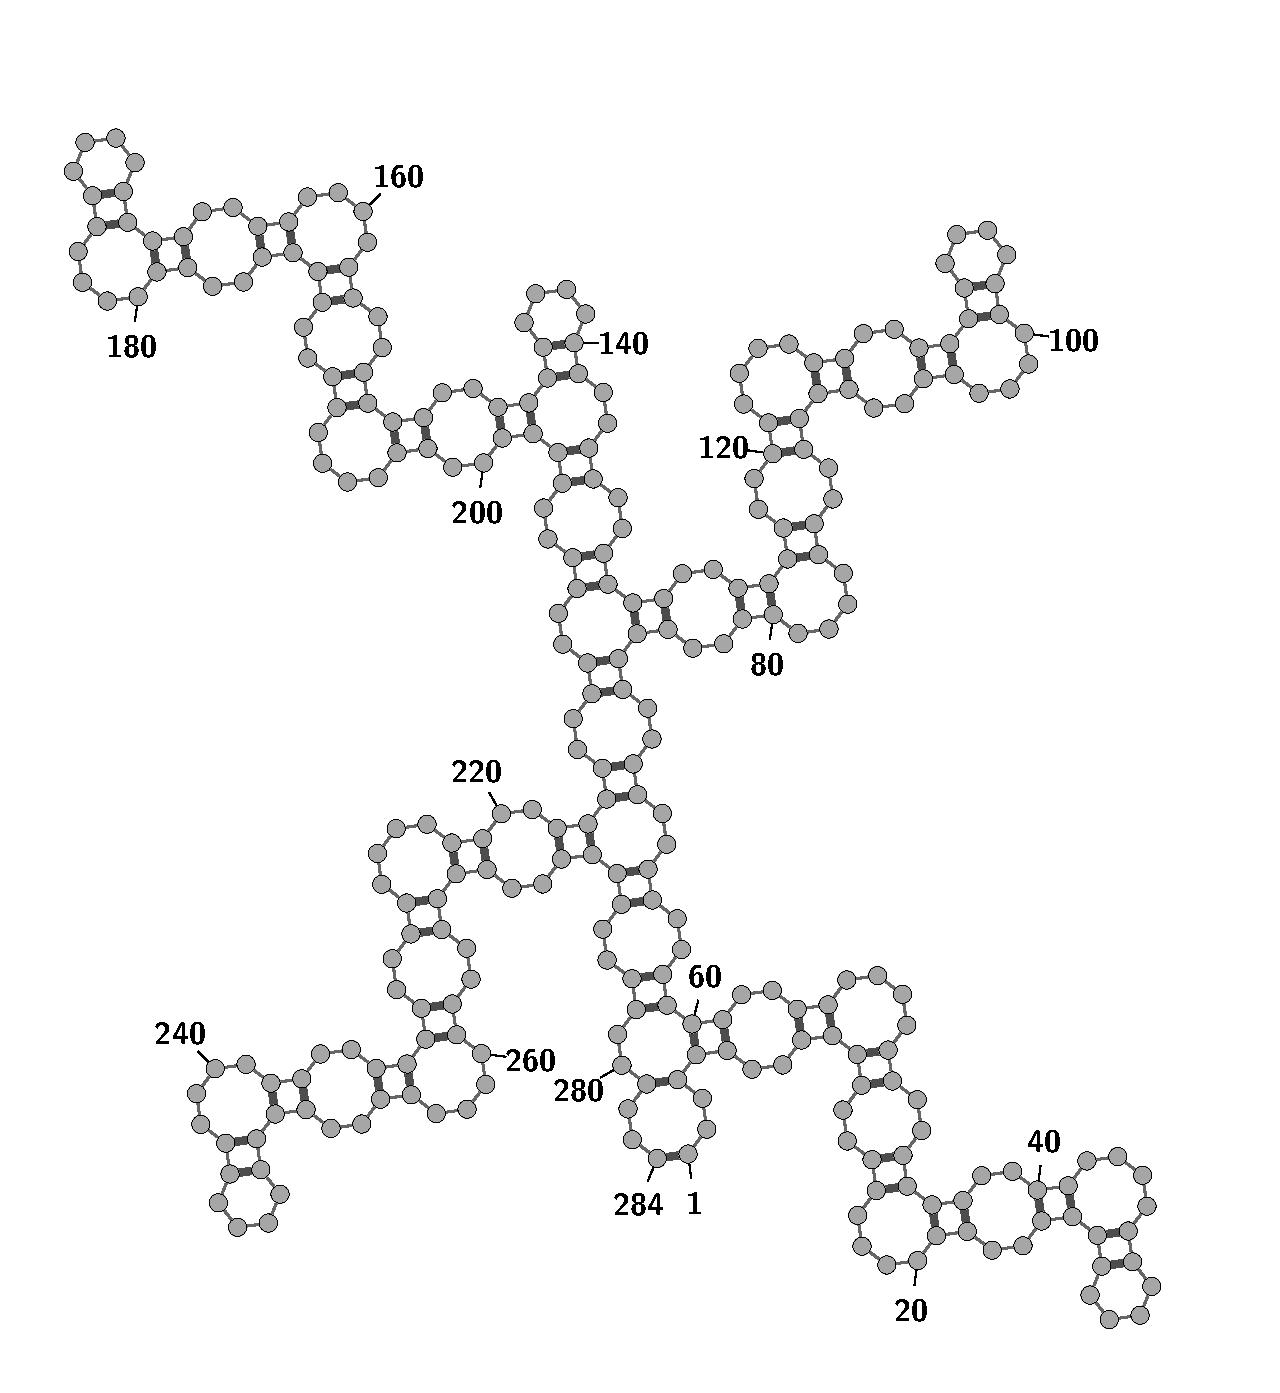
\includegraphics[width=0.45\linewidth]{figures/structures/target_78} &
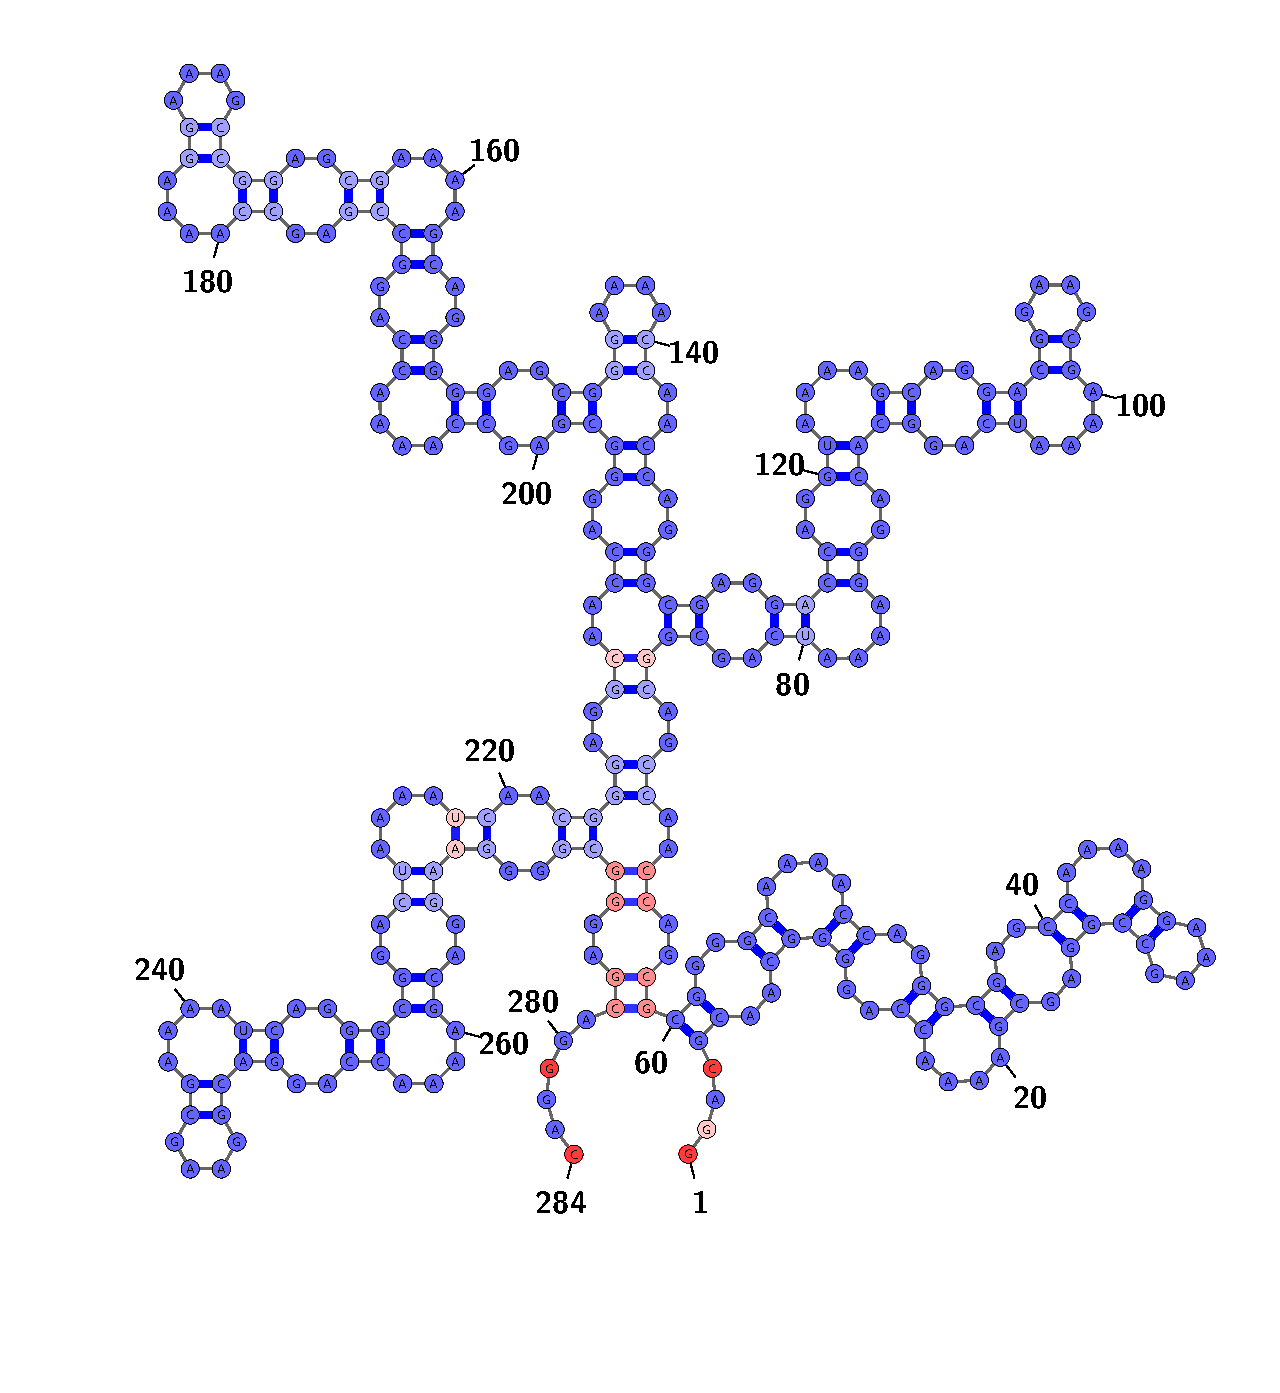
\includegraphics[width=0.45\linewidth]{figures/structures/structure_78_elite} \\[3pt]
(d) \MFE structure of SamplingDesign &
\begin{minipage}[t]{0.48\linewidth}\centering (e) Base-pairing probabilities, EliteDesign ($N=500$)\end{minipage} \\[1pt]
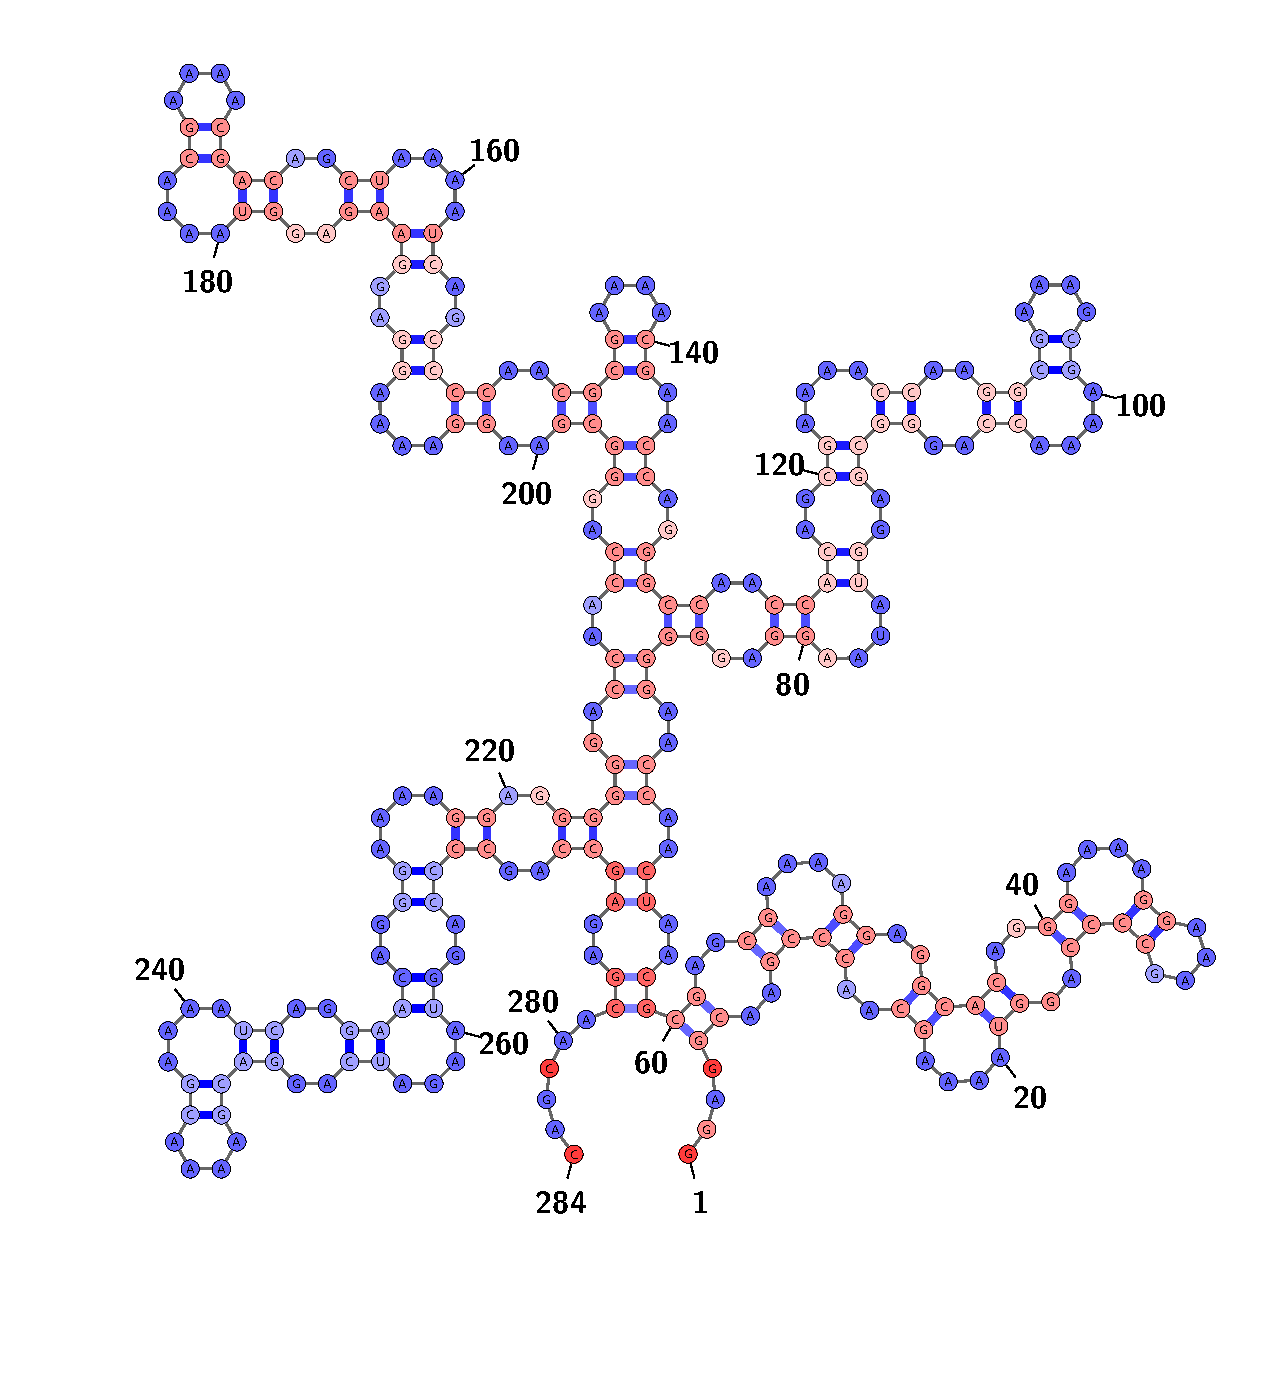
\includegraphics[width=0.45\linewidth]{figures/structures/structure_78_sampling} &
\begin{minipage}[b]{0.48\linewidth}\centering
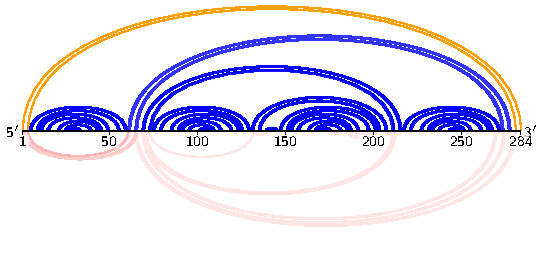
\includegraphics[width=\linewidth]{figures/structures/arcs_78_elite}\\[6pt]
(f) Base-pairing probabilities, SamplingDesign\\[1pt]
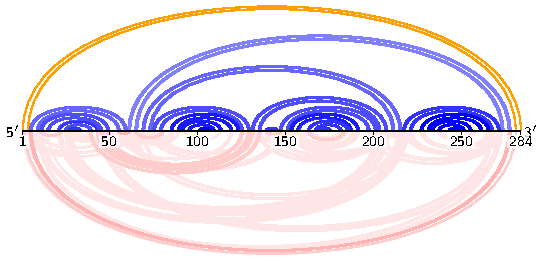
\includegraphics[width=\linewidth]{figures/structures/arcs_78_sampling}
\end{minipage}
\end{tabular}}
\captionof{figure}{}
\label{fig:eterna-structure-78}
\end{minipage}
